%% This is file `elsarticle-template-1-num.tex',
%%
%% Copyright 2009 Elsevier Ltd
%%
%% This file is part of the 'Elsarticle Bundle'.
%% ---------------------------------------------
%%
%% It may be distributed under the conditions of the LaTeX Project Public
%% License, either version 1.2 of this license or (at your option) any
%% later version.  The latest version of this license is in
%%    http://www.latex-project.org/lppl.txt
%% and version 1.2 or later is part of all distributions of LaTeX
%% version 1999/12/01 or later.
%%
%% Template article for Elsevier's document class `elsarticle'
%% with numbered style bibliographic references
%%
%% $Id: elsarticle-template-1-num.tex 149 2009-10-08 05:01:15Z rishi $
%% $URL: http://lenova.river-valley.com/svn/elsbst/trunk/elsarticle-template-1-num.tex $
%%

%% I need this here to get rid of the stupid "preprint submitted" shit on the front matter.
\documentclass[preprint,12pt]{elsarticle}
\makeatletter
\def\ps@pprintTitle{%
 \let\@oddhead\@empty
 \let\@evenhead\@empty
 \def\@oddfoot{}%
 \let\@evenfoot\@oddfoot}

%% Use the option review to obtain double line spacing
%% \documentclass[preprint,review,12pt]{elsarticle}

%% Use the options 1p,twocolumn; 3p; 3p,twocolumn; 5p; or 5p,twocolumn
%% for a journal layout:
%% \documentclass[final,1p,times]{elsarticle}
%% \documentclass[final,1p,times,twocolumn]{elsarticle}
%% \documentclass[final,3p,times]{elsarticle}
%% \documentclass[final,3p,times,twocolumn]{elsarticle}
%% \documentclass[final,5p,times]{elsarticle}
%% \documentclass[final,5p,times,twocolumn]{elsarticle}

%% The graphicx package provides the includegraphics command.
\usepackage{graphicx}
%% The amssymb package provides various useful mathematical symbols
\usepackage{amssymb}
%% The amsthm package provides extended theorem environments
%% \usepackage{amsthm}
\usepackage{qtree}
%% The lineno packages adds line numbers. Start line numbering with
%% \begin{linenumbers}, end it with \end{linenumbers}. Or switch it on
%% for the whole article with \linenumbers after \end{frontmatter}.
\usepackage{lineno}

\usepackage{color}
\usepackage{listings}
\definecolor{dkgreen}{rgb}{0,0.6,0}
\definecolor{gray}{rgb}{0.5,0.5,0.5}
\definecolor{mauve}{rgb}{0.58,0,0.82}
\definecolor{backcolour}{rgb}{1,0.95,0.84}


\lstset{
  language=R,
  backgroundcolor=\color{backcolour}, 
  aboveskip=3mm,
  belowskip=3mm,
  showstringspaces=false,
  columns=flexible,
  basicstyle={\small\ttfamily},
  numbers=none,
  numberstyle=\tiny\color{gray},
  keywordstyle=\color{blue},
  commentstyle=\color{dkgreen},
  stringstyle=\color{mauve},
  breaklines=true,
  breakatwhitespace=true,
  tabsize=3
}


%% natbib.sty is loaded by default. However, natbib options can be
%% provided with \biboptions{...} command. Following options are
%% valid:

%%   round  -  round parentheses are used (default)
%%   square -  square brackets are used   [option]
%%   curly  -  curly braces are used      {option}
%%   angle  -  angle brackets are used    <option>
%%   semicolon  -  multiple citations separated by semi-colon
%%   colon  - same as semicolon, an earlier confusion
%%   comma  -  separated by comma
%%   numbers-  selects numerical citations
%%   super  -  numerical citations as superscripts
%%   sort   -  sorts multiple citations according to order in ref. list
%%   sort&compress   -  like sort, but also compresses numerical citations
%%   compress - compresses without sorting
%%
%% \biboptions{comma,round}

% \biboptions{}

\journal{Mike}

\begin{document}

\begin{frontmatter}

%% Title, authors and addresses

\title{Predicting Baseball Hall Of Fame Inductions}

%% use the tnoteref command within \title for footnotes;
%% use the tnotetext command for the associated footnote;
%% use the fnref command within \author or \address for footnotes;
%% use the fntext command for the associated footnote;
%% use the corref command within \author for corresponding author footnotes;
%% use the cortext command for the associated footnote;
%% use the ead command for the email address,
%% and the form \ead[url] for the home page:
%%
%% \title{Title\tnoteref{label1}}
%% \tnotetext[label1]{}
%% \author{Name\corref{cor1}\fnref{label2}}
%% \ead{email address}
%% \ead[url]{home page}
%% \fntext[label2]{}
%% \cortext[cor1]{}
%% \address{Address\fnref{label3}}
%% \fntext[label3]{}


%% use optional labels to link authors explicitly to addresses:
%% \author[label1,label2]{<author name>}
%% \address[label1]{<address>}
%% \address[label2]{<address>}

\author{Michael Hirsch}
\address{ILLC, University of Amsterdam}
\address{michaelahirsch@gmail.com}

\begin{abstract}
%% Text of abstract
Every year, the Baseball Writers Association of America votes on a new Hall of Fame class. Each ballot consists of 10 votes, and players need to appear on 75\% of ballots in order to be inducted into the hall. Players have 15 years to get inducted, and are no longer eligible if that time period has passed. Here we attempt to classify hall of fame batters based on their career statistics using decision trees and an ensemble method, random forests.
\end{abstract}


\end{frontmatter}

%%
%% Start line numbering here if you want
%%
%% main text
\section{Introduction}
\label{S:1}
Major League Baseball (MLB) has been keeping thorough records of batting, picthing, and fielding statistics since its innagural season in 1869. Recently, with the advent of sabermetrics by the Society for American Baseball Research (SABR), many  new metrics building on traditional statistics were created. Such metrics caught the eye of stasticians, as these new metrics allowed for the creation of even more powerful predictive models. 

In this paper, we are investigating what makes a Hall Of Fame (HOF) batter. There have been over 20,000 Major League baseball players in the history of the organization, and only 211 of them have been inducted into the HOF. There are several ways in which a player can be inducted, and we only concern ourselves with players inducted from Baseball Writers Association of America (BBWAA) ballots, as this process is regulated. Often, fans and players feel that a worthy candidate is unfairly denied entry into the HOF because of voter bias, stacked ballots, or negative associations with performance enhancing drugs. The model proposed in this paper should be able account for these cases.

We will investigate predictions based on both classification trees and random forests. Random forests, introduced by Leo Breiman of UC Berkeley in 2001, is an ensemble learning technique that can be used for both classification and regression and improves on decision trees by correcting for overfitting. A random forest for classification consists of a collection of decision trees and outputs a prediction representing the most commonly occuring prediction of the decision trees.

\section{Data}
\label{S:2}
Data was collected from the Lahman Baseball Database, a freely available database that has been contiously updated since 1994 with the help of SABR and many individual researchers. There are many data tables available for download, but the ones that we are focusing on are \textit{Batting.dat} and \textit{HallOfFame.dat}. Batting statistics were supplied on a by-year basis, so a player's career statistics were computed by aggregating his yearly results. The batters' data was then merged with hall of fame voting results using the player's ID string. We will only be considering players who have appeared on at least one ballot, since failing to do so would indicate that that player is not hall worthy. All data preparation was done within R, the environment where we also build our learning models. 

Attention is paid to 12 different batting statistics over the course of the player's career:

\begin{enumerate}
	\item G: games played
	\item AB: at-bats
	\item R: runs
	\item H: hits
	\item X2B: doubles
	\item X3B: triples
	\item HR: homeruns
	\item RBI: runs batted in
	\item SB: stolen bases
	\item BB: walks
	\item SO: strike outs
	\item Inducted: classifier for HOF induction
\end{enumerate}

We needed to further filter our data by not including pitchers in our set of observations. This was done by removing those observations that indicated that the player recorded less than 300 RBI in his career. This number was not arbitrary, but rather chosen by cross referencing my data with HOF data from Baseball-Reference.

Our software of choice for this paper is R. We will be using several packages for our learning techniques, indicated in the sections below. Before training our model, it is important to have a quick look at our data.

\begin{figure}[h]
	\centering
	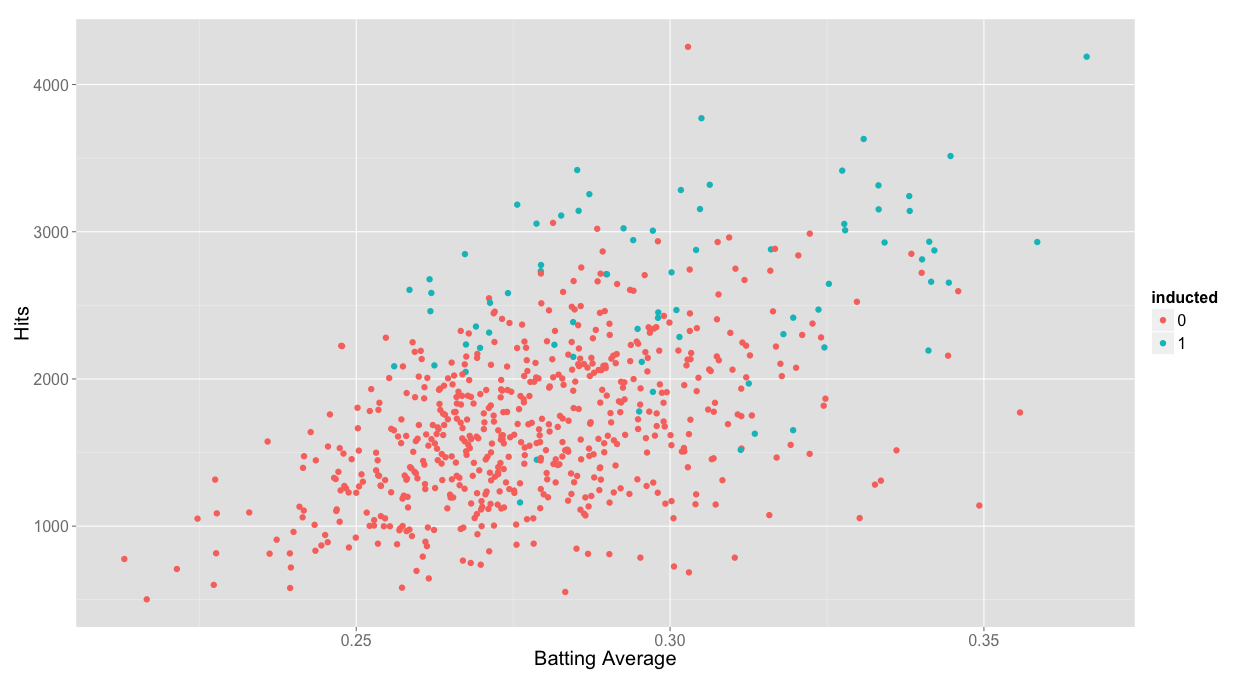
\includegraphics[width=1\textwidth]{BAandHits}
	\caption{Batters with more hits and a higher batting average are inducted}
\end{figure}

We can see that more hits and a higher batting average seem to correlate with induction. This makes sense, as one often judges the quality of a batter by his batting average, the numbers of hits a player has per at-bat.

\bigskip
\textbf{insert some more figures here}

% \begin{figure}[h]
% 	\centering
% 	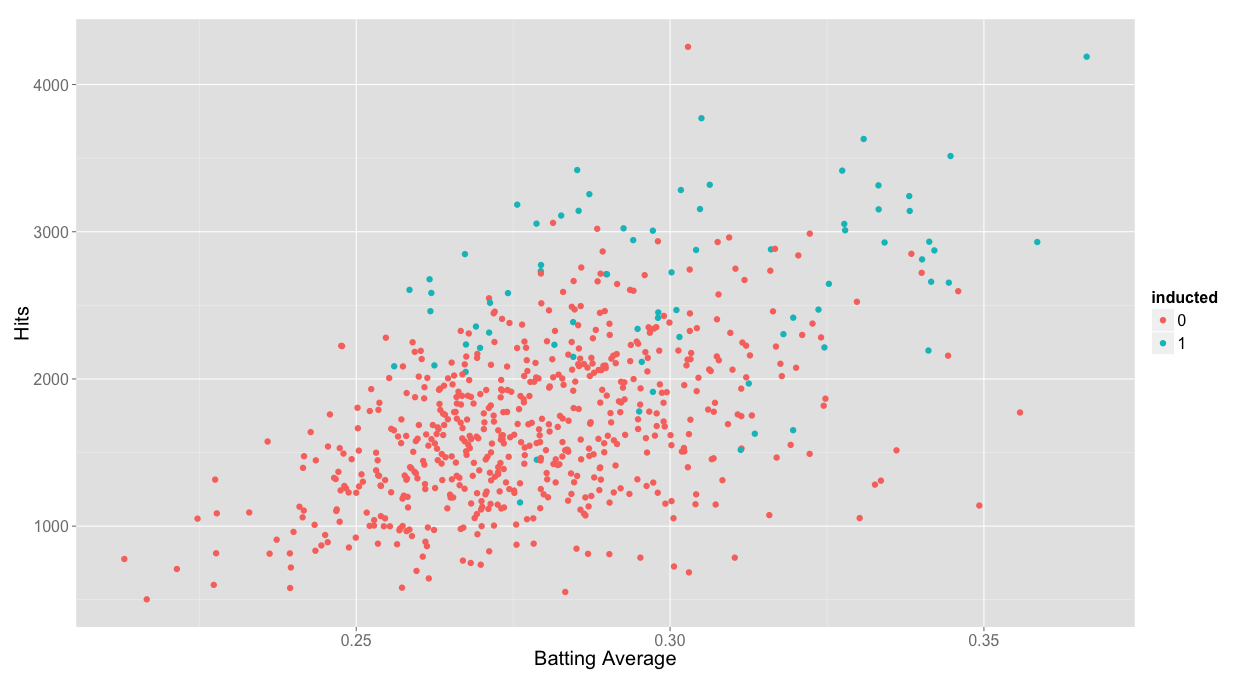
\includegraphics[width=1\textwidth]{BAandHits}
% 	\caption{Batters with more hits and a higher batting average are inducted}
% \end{figure}



% here is where we can add citations
%Maecenas \cite{Smith:2012qr} fermentum \cite{Smith:2013jd} urna ac sapien tincidunt 


\section{Tree-Based Methods for Classification}

In this section, we will give an account of two learning methods that we will use for the basis of prediction: classification trees, and an ensemble method, random forests. We will also introduce the concept of bootstrap aggregating (bagging) which is a fundamental ingredient of random forests. The information here is theoretical, and we will encounter applications of these ideas to our HOF data in the next section.

\subsection{Classification Trees}
Classification trees are a fairly effective predictive tool that are lauded for their high degree of interpretability. When constructing a classification tree, we begin with the full set of observations and begin dividing the predictor space into non-overlapping regions by means of binary splitting. In prediction, we assign each observation in a given region of the predictor space to the most commonly occuring class of the training observations in that region. 

\begin{figure}[h]
	\centering
	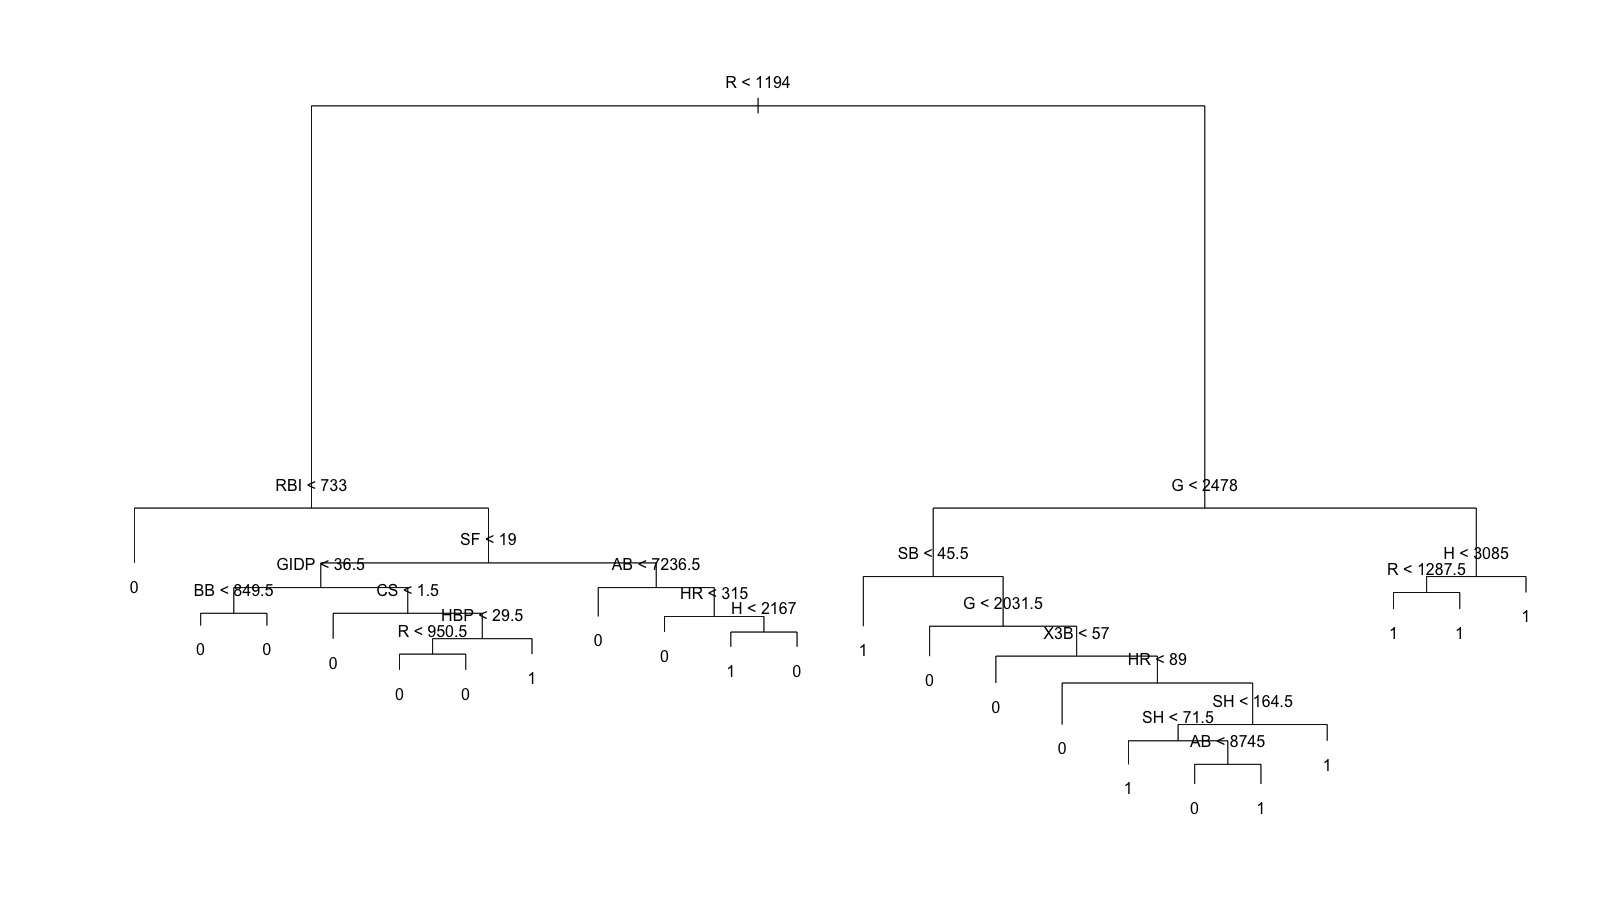
\includegraphics[width=1\textwidth]{Rplot}
	\caption{A very bushy classification tree}
\end{figure}

When choosing splits in our tree, we are concerned with the \textit{Gini Impurity} at each split, that is, we want to choose the feature to split on based on which feature split will give us the most pure sucessive node. Gini Impurity is a measure of how often a randomly chosen element from the set would be incorrectly labeled if it were randomly labeled according to the distribution of labels in the subset. Gini Impurity can be computed by summing the probability of each item being chosen times the probability of a mistake in categorizing that item. It reaches its minimum (zero)when all cases in the node fall into a single target category. This defined as:

$$G = \sum\limits_{k=1}^K \hat{p}_{mk}(1-\hat{p}_{mk}) = 1 - \sum\limits_{k=1}^K \hat{p}_{mk}^{2}$$

\noindent where $\hat{p}_{mk}$ denotes the proportion of training observations in the \textit{m}th region that are from the \textit{k}th class. So $G$ can be seen as a measure of total variance across the K classes. $G = 0$ when all observations in that region fall under on category. In splitting at nodes, we look to minimize this value.

Decision trees, while useful, have their limitations. Firstly, it is possible to grow overly complex trees that overfit the training data. In such cases, a method known as pruning (the specifics of which will not be covered in this paper) is required to combat this problem. Also, there are other methods by which binary splits can be determined, another popular one being \textit{information gain}, which is related to entropy. However, we concern ourselves only with \textit{Gini Impurity} since this is the method by which trees a generated using the \textit{trees} package in R.


\subsection{Ensemble Methods}
Ensemble methods use multiple learning algorithms to obtain better predictive performance than could be obtained from any of the individual learning algorithms composing the ensemble. Here, we look at two such methods, bagging and random forests.
\subsubsection{Tree Bagging}
Decision trees as discussed in the previous section often suffer from high variance, meaning that if we fit a decision tree to two random samples from a set of training observations, we could end up with vastly different results. Bagging is a method for reducing the variance of any learning method by taking repeated samples from a single training set and taking, in the case of classification, the most commonly occurring class among the boostrapped predictions. 

On average, each of the $B$ bootstrapped samples will take about two-thirds of the training observations.  The remaining observations that were not used in fitting a bagged tree are referred to as the \textit{out-of-bag} (OOB) observations, and we can predict the target varialbe for the \textit{i}th observation using each of the trees in which that observation was OOB. This will yield, on average, $B/3$ predictions from which we can predict the classification for the observation by taking majority vote. Using this method, we can get a single OOB prediction for each of our observations, obtaining an OOB error, which is a valid estimate of the test error for our bagged model.

Bagging also gives us insight into which of our predictors were the most important in creating our model by looking at the Gini Impurity. To do so, we take the sum of the amount that Gini Impurity has dereased by splitting on a given predictor and take the average over our $B$ trees.

\subsubsection{Random Forest}
The random forest technique is quite similar to taking bagged  samples of trees, with the main difference being that at each of the splits only a random sample $m$ of the set of all predictors $p$ is considered. Typically, $m \approx \sqrt{p}$ predictors suffice. This technique helps to decorrelate the tree, as there may be one predictor that has a very high influence in classification. In the case of bagging, this predictor will most likely be used as the first split in a majority of the trees, causing most bagged trees to be quite similar and correlated. By forcing each split to consider on a subset of the predictors, on average $(p-m)/p$ of the splits will not consider this strong predictor.


% \begin{table}[h]
% \centering
% \begin{tabular}{l l l}
% \hline
% \textbf{Treatments} & \textbf{Response 1} & \textbf{Response 2}\\
% \hline
% Treatment 1 & 0.0003262 & 0.562 \\
% Treatment 2 & 0.0015681 & 0.910 \\
% Treatment 3 & 0.0009271 & 0.296 \\
% \hline
% \end{tabular}
% \caption{Table caption}
% \end{table}


\begin{figure}[h]
	\centering
	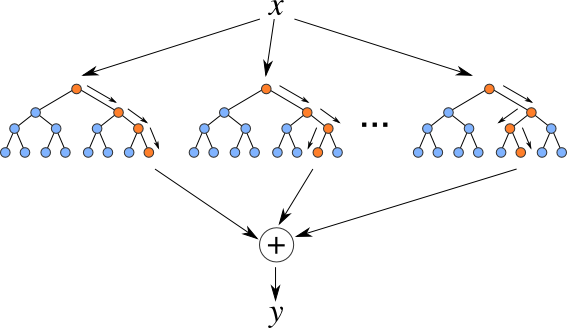
\includegraphics[width=1\textwidth]{RF}
	\caption{A Random Forest. The prediction for \textbf{y} is made by majority vote. \textbf{get a new figure}}
\end{figure}

In this paper, we will be utiliziing the \textit{randomForest} package in R. 

\section{Prediction Models}

In this section, we apply the techniques introduced in the last section to our HOF data. We will start by creating a single decision tree based on some training data, and then predicting the induction classifier of our training data based on our model. We will also look at some metrics that will allow us to test the effectiveness of our classification models in order to see what parameters would be best to use. 

After evaluating our single decision tree, we will move onto random forest classification, to see how it improves our predictions. 

\subsection{Classification Tree}
Using R's tree package, we can fit a classification tree to our data. To do so, we will split the entire data set into a training and a test set and build our tree using the training data. As our training set, we will take a random sample of about $2/3$ of our data. This amounts to $\approx 400$ observations.
The following results were obtained by predicting induction based on all of our features except for playerID. The tree determined that runs, stolen bases, strikeouts, walks, home runs, grounded into double plays, at-bats, and hit by pitches were the most important features. We also see that the tree has a misclassification rate of $3.25\%$ A quick look at the tree indicates that the number of runs a player has scored in his career is the most important predictor, since the first split was made usings runs. This is not surpising, as runs are one of the only statistics that we considered that relate directly to a player's team winning a game. 
\bigskip

\begin{figure}[h1]
	\centering
	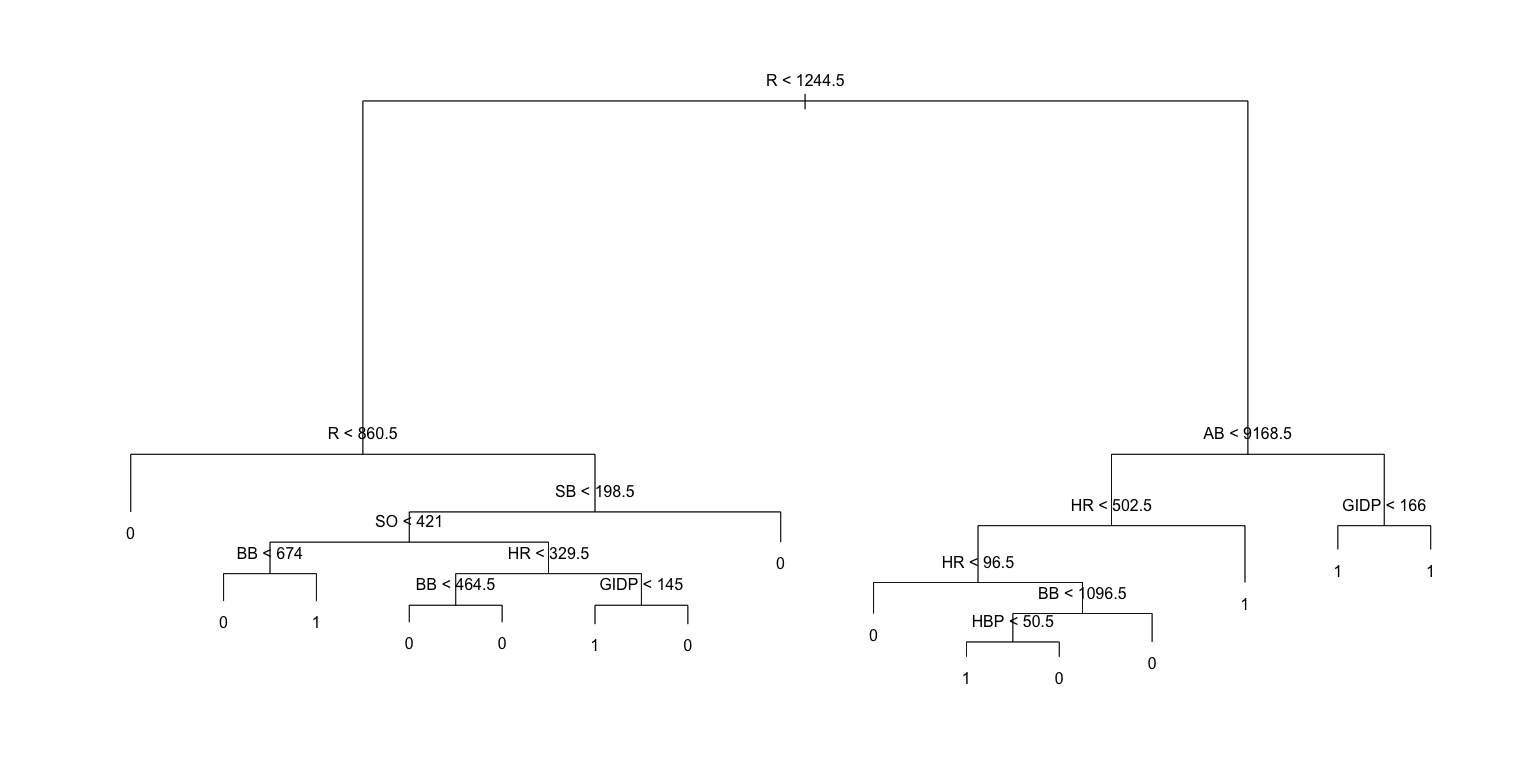
\includegraphics[width=0.9\textwidth]{MachineLearnTree}
	\caption{An unpruned tree}
\end{figure}

\begin{lstlisting}
Classification tree:
tree(inducted ~ . - playerID, data = HallOfFame, subset = train)
Variables actually used in tree construction:
[1] "R"    "SB"   "SO"   "BB"   "HR"   "GIDP" "AB"   "HBP" 
Number of terminal nodes:  15 
Misclassification error rate: 0.0325 = 13 / 400 
\end{lstlisting}


Now, to test the performance of this tree, we must estimate a test error by predicting a player's hall of fame induction on our test data. We will look at how our classification model performed.

\begin{lstlisting}
tree.pred=predict(tree.hof,HallOfFame[-train,],type="class")
with(HallOfFame[-train,],table(tree.pred,inducted))
         inducted
tree.pred   0   1
        0 203  11
        1  19  18
\end{lstlisting}

This tells us that we have a misclassification rate of $1-(203+18)/(203+18+11+19) \approx 12\%$. We will see if this can be improved by using the tree package's pruning feature. The goal of pruning a decision tree is to reduce the complexity of our model, and to reduce overfitting. A pruned tree is simply a less complex tree chosen from set of all subtrees of our decision tree. The method used by the tree package in R is \textit{cost complexity pruning}, which operates as follows: Rather than considering every subtree of our initial tree, we only consider a sequence of trees that is indexed by a tuning parameter $\alpha$. The goal of pruning is to select a subtree that will lead to the lowest misclassification error rate. Such an $\alpha$ can be chosen by using cross-validation on our initial tree.\textbf{talk about cv and pruning more?}



\noindent We can see that the optimal size for a tree is between 4 and 7 terminal nodes. With this imformation, we can prune back our original tree to have a more interpretable and accurate model.

\begin{lstlisting}
Classification tree:
snip.tree(tree = tree.hof, nodes = c(7L, 2L))
Variables actually used in tree construction:
[1] "R"  "AB" "HR" "BB" "G" 
Number of terminal nodes:  7 
Misclassification error rate: 0.04 = 16 / 400 

         inducted
tree.pred   0   1
        0 207  10
        1  15  19
\end{lstlisting}

\begin{figure}[h2]
	\centering
	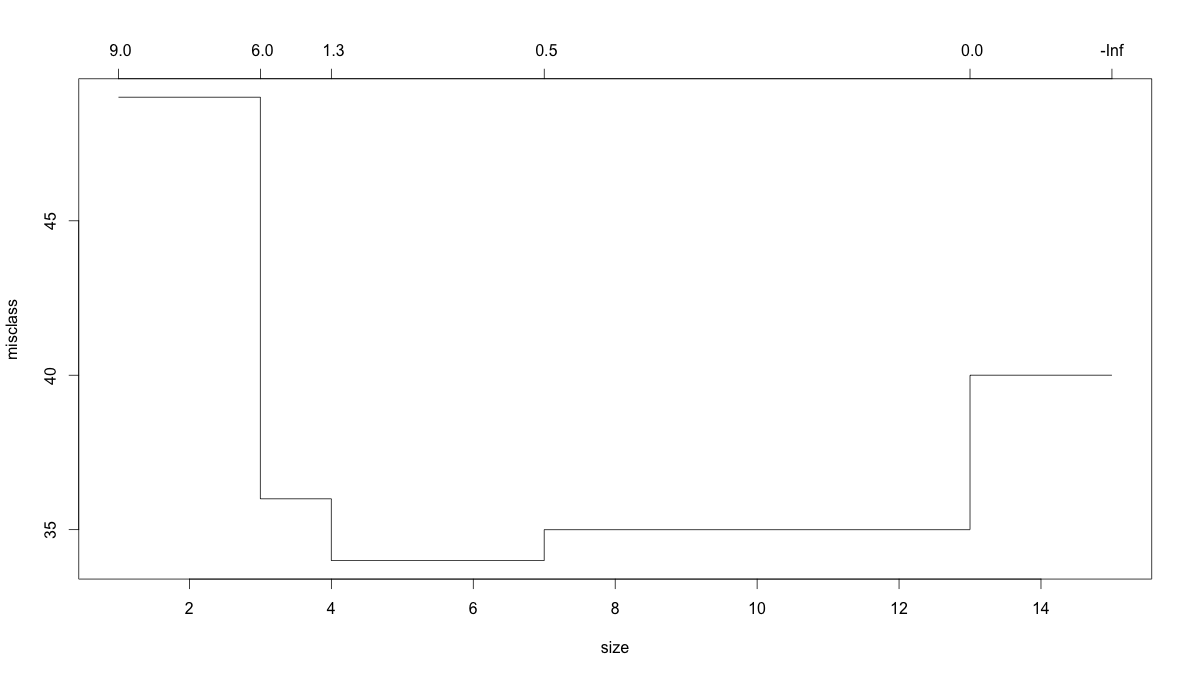
\includegraphics[width=0.9\textwidth]{pruneCV}
	\caption{Tree size against misclassification}
\end{figure}

\begin{figure}[h3]
	\centering
	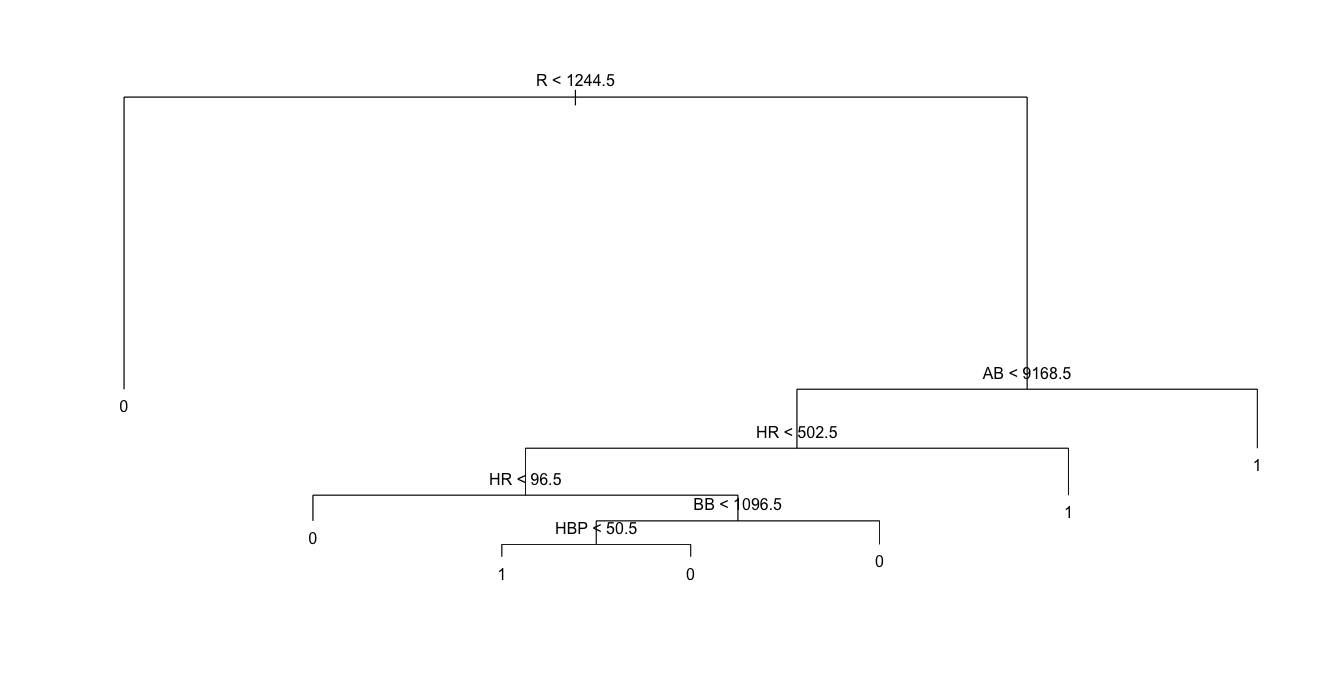
\includegraphics[width=0.9\textwidth]{pruned}
	\caption{Our pruned tree with 7 terminal nodes}
\end{figure}


\subsection{Random Forest}

\section{Conclusions}

% \begin{table}[h]
% \centering
% \begin{tabular}{l l l}
% \hline
% \textbf{Treatments} & \textbf{Response 1} & \textbf{Response 2}\\
% \hline
% Treatment 1 & 0.0003262 & 0.562 \\
% Treatment 2 & 0.0015681 & 0.910 \\
% Treatment 3 & 0.0009271 & 0.296 \\
% \hline
% \end{tabular}
% \caption{Table caption}
% \end{table}


%% References
%%
%% Following citation commands can be used in the body text:
%% Usage of \cite is as follows:
%%   \cite{key}          ==>>  [#]
%%   \cite[chap. 2]{key} ==>>  [#, chap. 2]
%%   \citet{key}         ==>>  Author [#]

%% References with bibTeX database:

\bibliographystyle{model1-num-names}
\bibliography{sample.bib}

%% Authors are advised to submit their bibtex database files. They are
%% requested to list a bibtex style file in the manuscript if they do
%% not want to use model1-num-names.bst.

%% References without bibTeX database:

% \begin{thebibliography}{00}

%% \bibitem must have the following form:
%%   \bibitem{key}...
%%

% \bibitem{}

% \end{thebibliography}


\end{document}

%%
%% End of file `elsarticle-template-1-num.tex'.